\section{Decimals and fractions 小数与分数}
\subsection{Decimals 小数}
\begin{paracol}{2}
Decimals is a representation of a non-negative real numbers. The dots in the number is called decimal separator. A decimal separator is a symbol used to separate the integer part from the fractional part of a number written in decimal form.
\switchcolumn
小数,是实数的一种特殊的表现形式。小数中的圆点叫做小数点,它是一个小数的整数部分和小数部分的分界号。其中整数部分是零的小数叫做纯小数,整数部分不是零的小数叫做带小数。
\end{paracol}

\begin{figure}[!hbtp]
\begin{center}
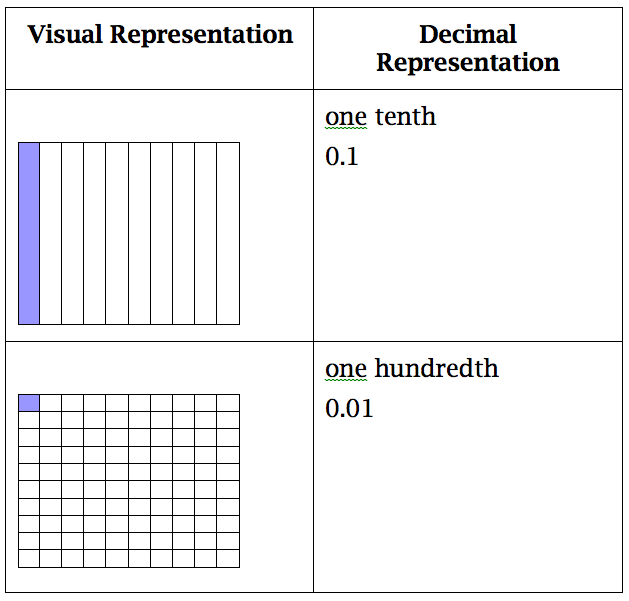
\includegraphics[width=0.6\textwidth]{tenth.png}
      \caption{Visual representation of decimals and fractions 小数和分数的图像表示}
      \label{fig:decimalsquare}
\end{center}
\end{figure}

\begin{table}[htp]
\centering
\begin{tabular}{|p{.8cm}<{\centering}|p{.8cm}<{\centering}|p{.8cm}<{\centering}|p{.8cm}<{\centering}!{\vrule width 1.6pt}p{.8cm}<{\centering}|p{.8cm}<{\centering}|p{.8cm}<{\centering}|}
\hline
\parbox[t]{2mm}{\rotatebox[origin=c]{90}{thousands} }&
\parbox[t]{2mm}{\rotatebox[origin=c]{90}{hundred}}&\parbox[t]{2mm}{ \rotatebox[origin=c]{90}{ten}}& \parbox[t]{2mm}{\rotatebox[origin=c]{90}{ones} }&
\rotatebox[origin=c]{90}{\parbox[c]{2cm}{\centering \begin{spacing}{0.8}tenths\end{spacing}}}&\rotatebox[origin=c]{90}{\parbox[c]{2cm}{\centering \begin{spacing}{0.8}hundredths\end{spacing}}}& \rotatebox[origin=c]{90}{\parbox[c]{2cm}{\centering thousandths}}\\
\midrule
7&5&5&0&2&6&2\\
\bottomrule
\end{tabular}
\caption{7550.262: Seven thousand five hundred fifty and two hundred sixty-two thousandths\\
七千五百五十五又千分之二百六十二\label{tab:decimals}}
\end{table}

\begin{paracol}{2}
\begin{description}
\item [{\bf Finite decimals: }] A regular number, also called a finite decimal, is a positive number that has a finite decimal expansion,like $3.1465$,$0.364$,$8.3218798456$, and so on. 
\item [{\bf Repeating decimals: }] A repeating decimal, \\
 also called a recurring decimal, is a number whose decimal representation eventually becomes periodic (i.e., the same sequence of digits repeats indefinitely), like $0.\overline{142857}=0.142857142857\ldots$ and $1.8\overline{3}=1.833\ldots$. The minimum number of digits that repeats in such a number is known as the decimal period. 
\item [{\bf Nonperiodic and nonrepeating decimals: }] \ \\ Nonperiodic and nonrepeating decimal is an irrational number. An irrational number is a number that cannot be expressed as a fraction. For example, the ratio of a circle's circumference to its diameter is $\pi =3.141592653589793\ldots$.  Euler's number is $e=2.71828\ldots$.
\end{description}
\switchcolumn
\begin{description}
\item [{\bf 有限小数:}] 小数部分后有有限个数位的小数。如$3.1465$,$0.364$,$8.3218798456$等。\\ 
%有限小数都属于有理数,可以化成分数形式。
%一个最简分数可以被化作十进制的有限小数当且仅当其分母只含有质因数2或5或两者。 类似的,一个最简分数可以被化作某正整数底数的有限小数当且仅当其分母之质因数为此基底质因数的子集。
\item [{\bf 循环小数:}] 从小数部分的某一位起,一个数字或几个数字,依次不断地重复出现的小数叫做循环小数。如 $0.\overline{142857}=0.142857142857\ldots$,$1.8\overline{3}=1.833\ldots$等。这一节数字称为循环节。\\ \\ \\ \\  %循环小数亦属于有理数,可以化成分数形式。
\item [{\bf 无限不循环小数:}] 小数部分有无限多个数字,且没有依次不断地重复出现的一个数字或几个数字的小数叫做无限不循环小数,如圆周率 $\pi =3.14159265358979323\ldots$,自然对数的底数 $e=2.71828182845904\ldots$。%无限不循环小数也就是无理数,不能化成分数形式。
\end{description}
\end{paracol}

\subsection{Fractions 分数}

\begin{paracol}{2}
A fraction represents a part of a whole or, more generally, any number of equal parts. A fraction (examples:  $\frac{1}{2}$ and $17/3$) consists of an numerator displayed above a line (or before a slash), and a non-zero denominator. The numerator represents a number of equal parts, and the denominator indicates how many of those parts make up a unit or a whole. 
\switchcolumn
分数可视为将某件事物平均分成的几份中占据其中的几份。分数可以用分式来表示,例如 $\frac{1}{2}$ 和 $17/3$。其中,中间的线称为分数线。分数线上的称为分子,分数线下的数称为分母。
\end{paracol}

\begin{paracol}{2}
\begin{description}
\item [{\bf Irreducible fraction:}] An irreducible fraction is a fraction in which the numerator and denominator are integers that have no other common divisors than 1.
\item [{\bf Proper Fraction: }] The fraction is called proper if the numerator is less than the denominator. In general, a common fraction is said to be a proper fraction if the absolute value of the fraction is strictly less than one.
\item [{\bf Top-heavy/Improper Fraction: }] It is said to be an improper fraction, or sometimes top-heavy fraction,[12] if the absolute value of the fraction is greater than or equal to 1.
\item [{\bf mixed numeral: }] A mixed numeral is a traditional denotation of the sum of a non-zero integer and a proper fraction. Any such mixed fractions can be converted to an improper fraction. For example, $1\frac{1}{2}=\frac{1\times2+1}{2}=\frac{3}{2}$.
\item [{\bf unit fraction: }] A unit fraction is a number written as a fraction where the numerator is one and the denominator is a positive integer.
\end{description}
\switchcolumn
\begin{description}
\item [{\bf 最简分数(既约分数):}] 分子是整数,分母是正整数,且分子和分母互素的分数。\\ 
\item [{\bf 真分数:}] 除商小于1、大于0的分数,即分子小于分母的分数。\\ \\ \\ \\ 
\item [{\bf 假分数:}] 假分数是指除商不小于1的分数,即分子等于或大于分母的分数。\\ \\ \\ 
\item [{\bf 带分数:}] 一个整数加一个真分数,带分数可以写成假分数。例如 $1\frac{1}{2}$,就是一又二分之一,与$\frac{1\times2+1}{2}=\frac{3}{2}$等价。\\ \\ \\ 
\item [{\bf 单位分数:}] 分子为1,分母是整数的分数。
\end{description}
\end{paracol}

\paragraph{Equivalent fractions 约分、扩分及通分}
\ \ \\

\begin{paracol}{2}
Multiplying the numerator and denominator of a fraction by the same (non-zero) number results in a fraction that is equivalent to the original fraction. This is true because multiplying the numerator and denominator of a fraction by the same number is equivalent to multiplying by one, and any number multiplied by one has the same value as the original number. Dividing the numerator and denominator of a fraction by the same non-zero number will also yield an equivalent fraction. This is called reducing or simplifying the fraction. A common fraction can be reduced to lowest terms by dividing both the numerator and denominator by their greatest common divisor.
\switchcolumn
\ \\ 一个分数约分后或扩分后,其分数与原来之分数的值相等,称为等值分数。“扩分”是将一个分数的分子和分母同乘以比1大的数。 扩分后的分数和原来分数的值相等。“约分”是将一个分数的分子和分母同除以一个比1大的整数(它们的公约数)。 约分后的分数和原来分数的值相等。“通分”是利用约分或扩分,将两个分母不同的分数,分别化为同分母的分数。
\end{paracol}

\subsection{Converting between decimals and fractions 小数与分数的转化}

\begin{paracol}{2}
To change a common fraction to a decimal, do a long division of the decimal representations of the numerator by the denominator (this is idiomatically also phrased as "divide the denominator into the numerator"), and round the answer to the desired accuracy. To change a decimal to a fraction, we need to consider by the different types of decimals.
\switchcolumn[1]
把分数化为小数只需要做一个除法。用分子除以分母,然后取到小数点后相应的位数。根据小数类型的不同,有不同的方法把小数化为分数:
\switchcolumn[0]*
\begin{description}
\item [{\bf Convert finite decimals: }] To change a decimal to a fraction, write in the denominator a  $1$ followed by as many zeroes as there are digits to the right of the decimal point, and write in the numerator all the digits of the original decimal, just omitting the decimal point. For example, $12.3456 = \frac{123456}{10000}$.
\item [{\bf Converting repeating decimals to fractions}] For repeating patterns where the repeating pattern begins immediately after the decimal point, a simple division of the pattern by the same number of nines as numbers it has will suffice. For example, $0.\overline{9}=\frac{9}{9}=1$, $0.\overline{25}=\frac{25}{99}$, $0.\overline{3}=\frac{3}{9}=\frac{1}{3}$. In case leading zeros precede the pattern, the nines are suffixed by the same number of trailing zeros. In case a non-repeating set of decimals precede the pattern, we can write it as the sum of the non-repeating and repeating parts, respectively:
$0.1\overline{3}=0.1+0.0\overline{3}=\frac{3}{30}+\frac{1}{10}\frac{1}{3} = \frac{4}{30} = \frac {2}{15}$.
\item [{\bf Nonperiodic and nonrepeating decimals}] \ \\ Nonperiodic and nonrepeating decimal is an irrational number. Therefore, it cannot be converted to a fraction. 
\end{description} 
\switchcolumn
\begin{description}
\item [{\bf 有限小数化分数:}] 把有限小数去掉小数点后作为分子;分母是以“1”开头,有限小数的小数点后有几位,就在1后跟几个零。例如:$12.3456 = \frac{123456}{10000}$。\\ \\ \\ \\ 
\item [{\bf 循环小数化分数:}] 如果是纯循环小数则把循环节作为分子,循环节如果有一位,分母为9;循环节有两位,分母为99;循环节有三位,分母为999,依次类推。如 $0.\overline{9}=\frac{9}{9}=1$,$0.\overline{25}=\frac{25}{99}$, $0.\overline{3}=\frac{3}{9}=\frac{1}{3}$。混循环小数化分数则需要化为有限小数和纯循环小数之和后化简,如 $0.1\overline{3}=0.1+0.0\overline{3}=\frac{3}{30}+\frac{1}{10}\frac{1}{3} = \frac{4}{30} = \frac {2}{15}$。\\ \\ \\ \\ \\ \\ 
\item [{\bf 无限不循环小数}] 无限不循环小数为无理数,不可以化为分数。
\end{description}
\end{paracol}

\newpage
